\section {Taxonomic-key diagram}           \label{sec:choosingVirtualizationTechnology}
	\begin{figure*}[ht]
		\centering
		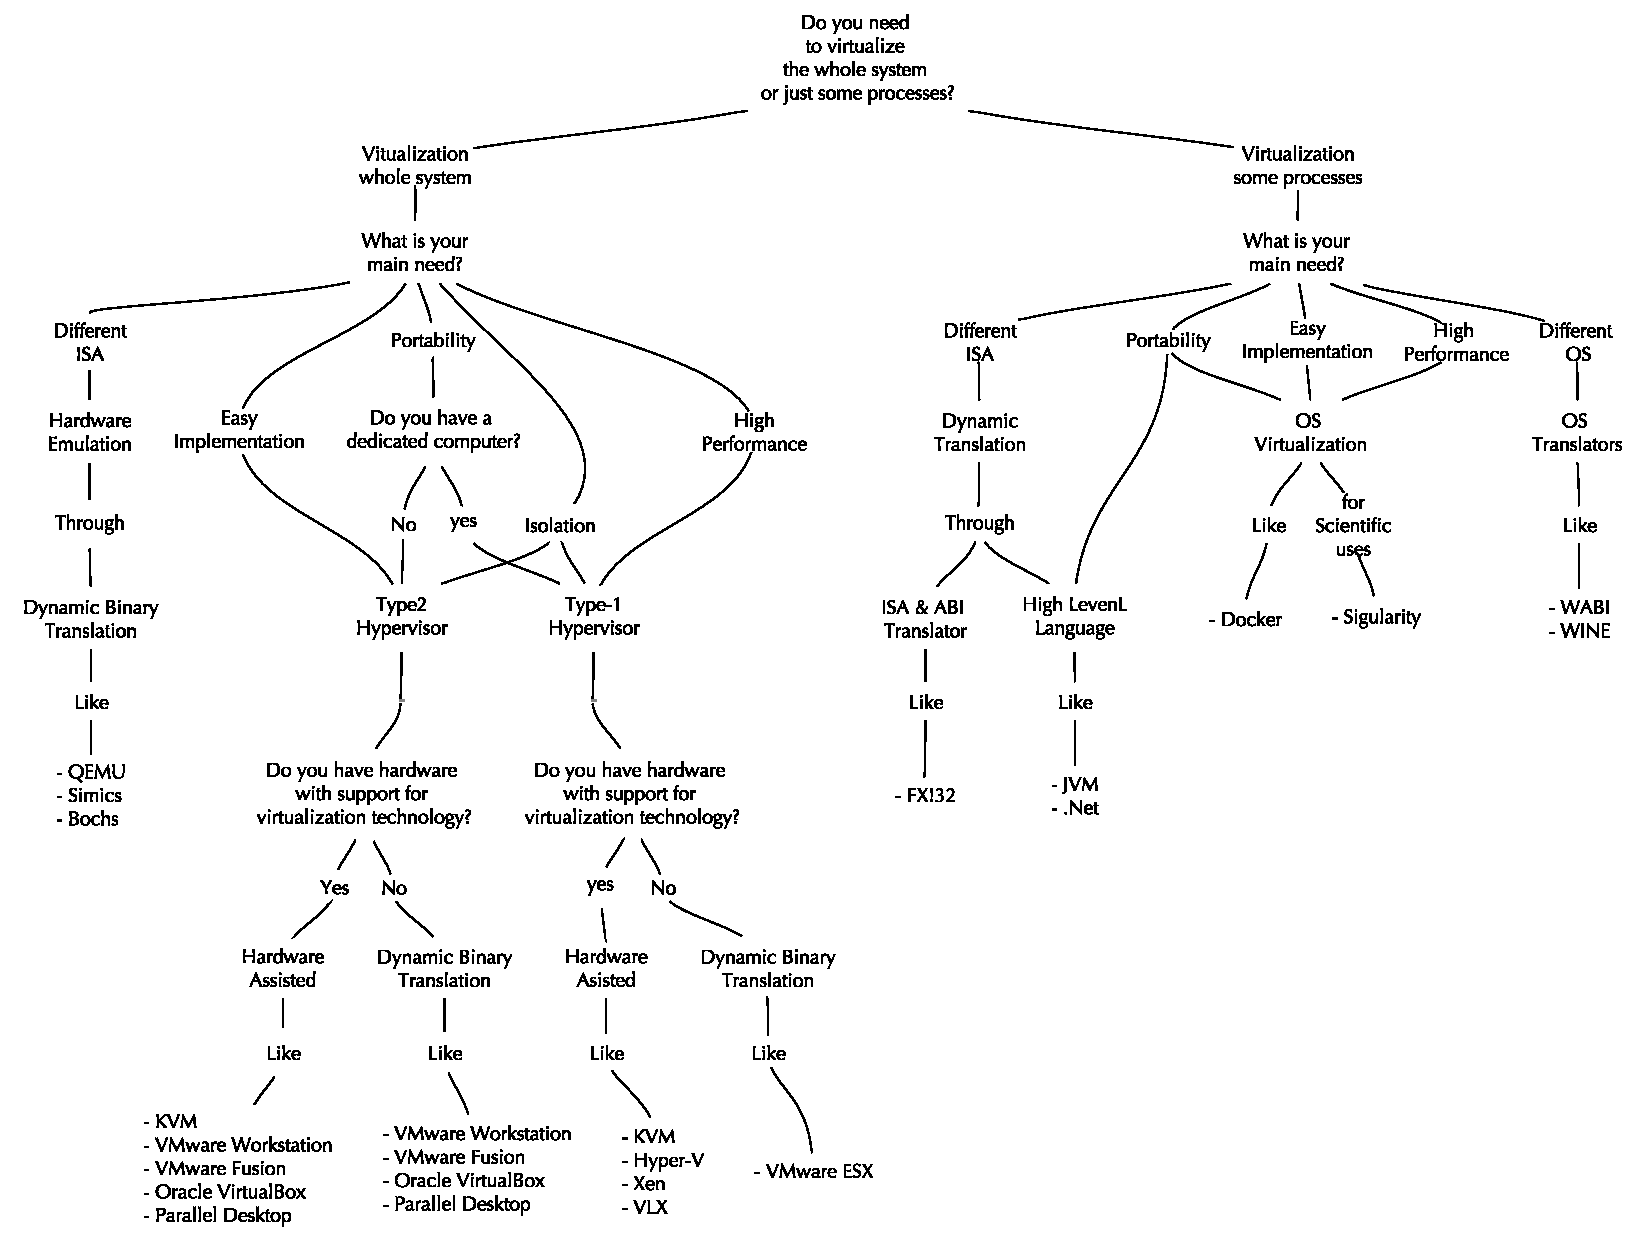
\includegraphics[width=18cm]{images/taxonomic-KeyDiagramV2.pdf}
		\vspace{-0.2cm}
		\caption{Taxonomic key diagram for the selection of virtualization technologies.}
		\label{fig:taxonomic-keyDiagram}
	\end{figure*}
	
	In this paper, we also propose a second element that consists of a \textit{taxonomic-key diagram}, similar to the dichotomous keys used in Biology. The purpose of this diagram is to guide decision making about the technologies related to the virtual machines as indicated in the proposed taxonomy, see Figure \ref{fig:taxonomic-keyDiagram}. The diagram uses a set of questions, which, depending on each possibility of response,  establishes a path that leads to the identification of a type of virtual machine technology defined in the previous taxonomy. For example, the diagram can be used by asking the question, Do you need to virtualize the entire system or just some of its processes? If the complete system needs to be virtualized, the following question will inquire about the specific need. If the desired virtual system needs an ISA different from the underlying hardware, the answer from the taxonomic-key is set the category \textit {Dynamic Binary Translation}, for example; \textit{QEMU}, \textit{Simics} and \textit{Bochs}. 
